\section{Checkpoints}

In order to avoid sources of frustration for the player, avoiding to repeat parts of the level he already successfully completed, and, sometimes, even let him change his mind about the choices he has taken, we have inserted checkpoints in safe zones along the way.
\begin{figure}[H]
  \centering
  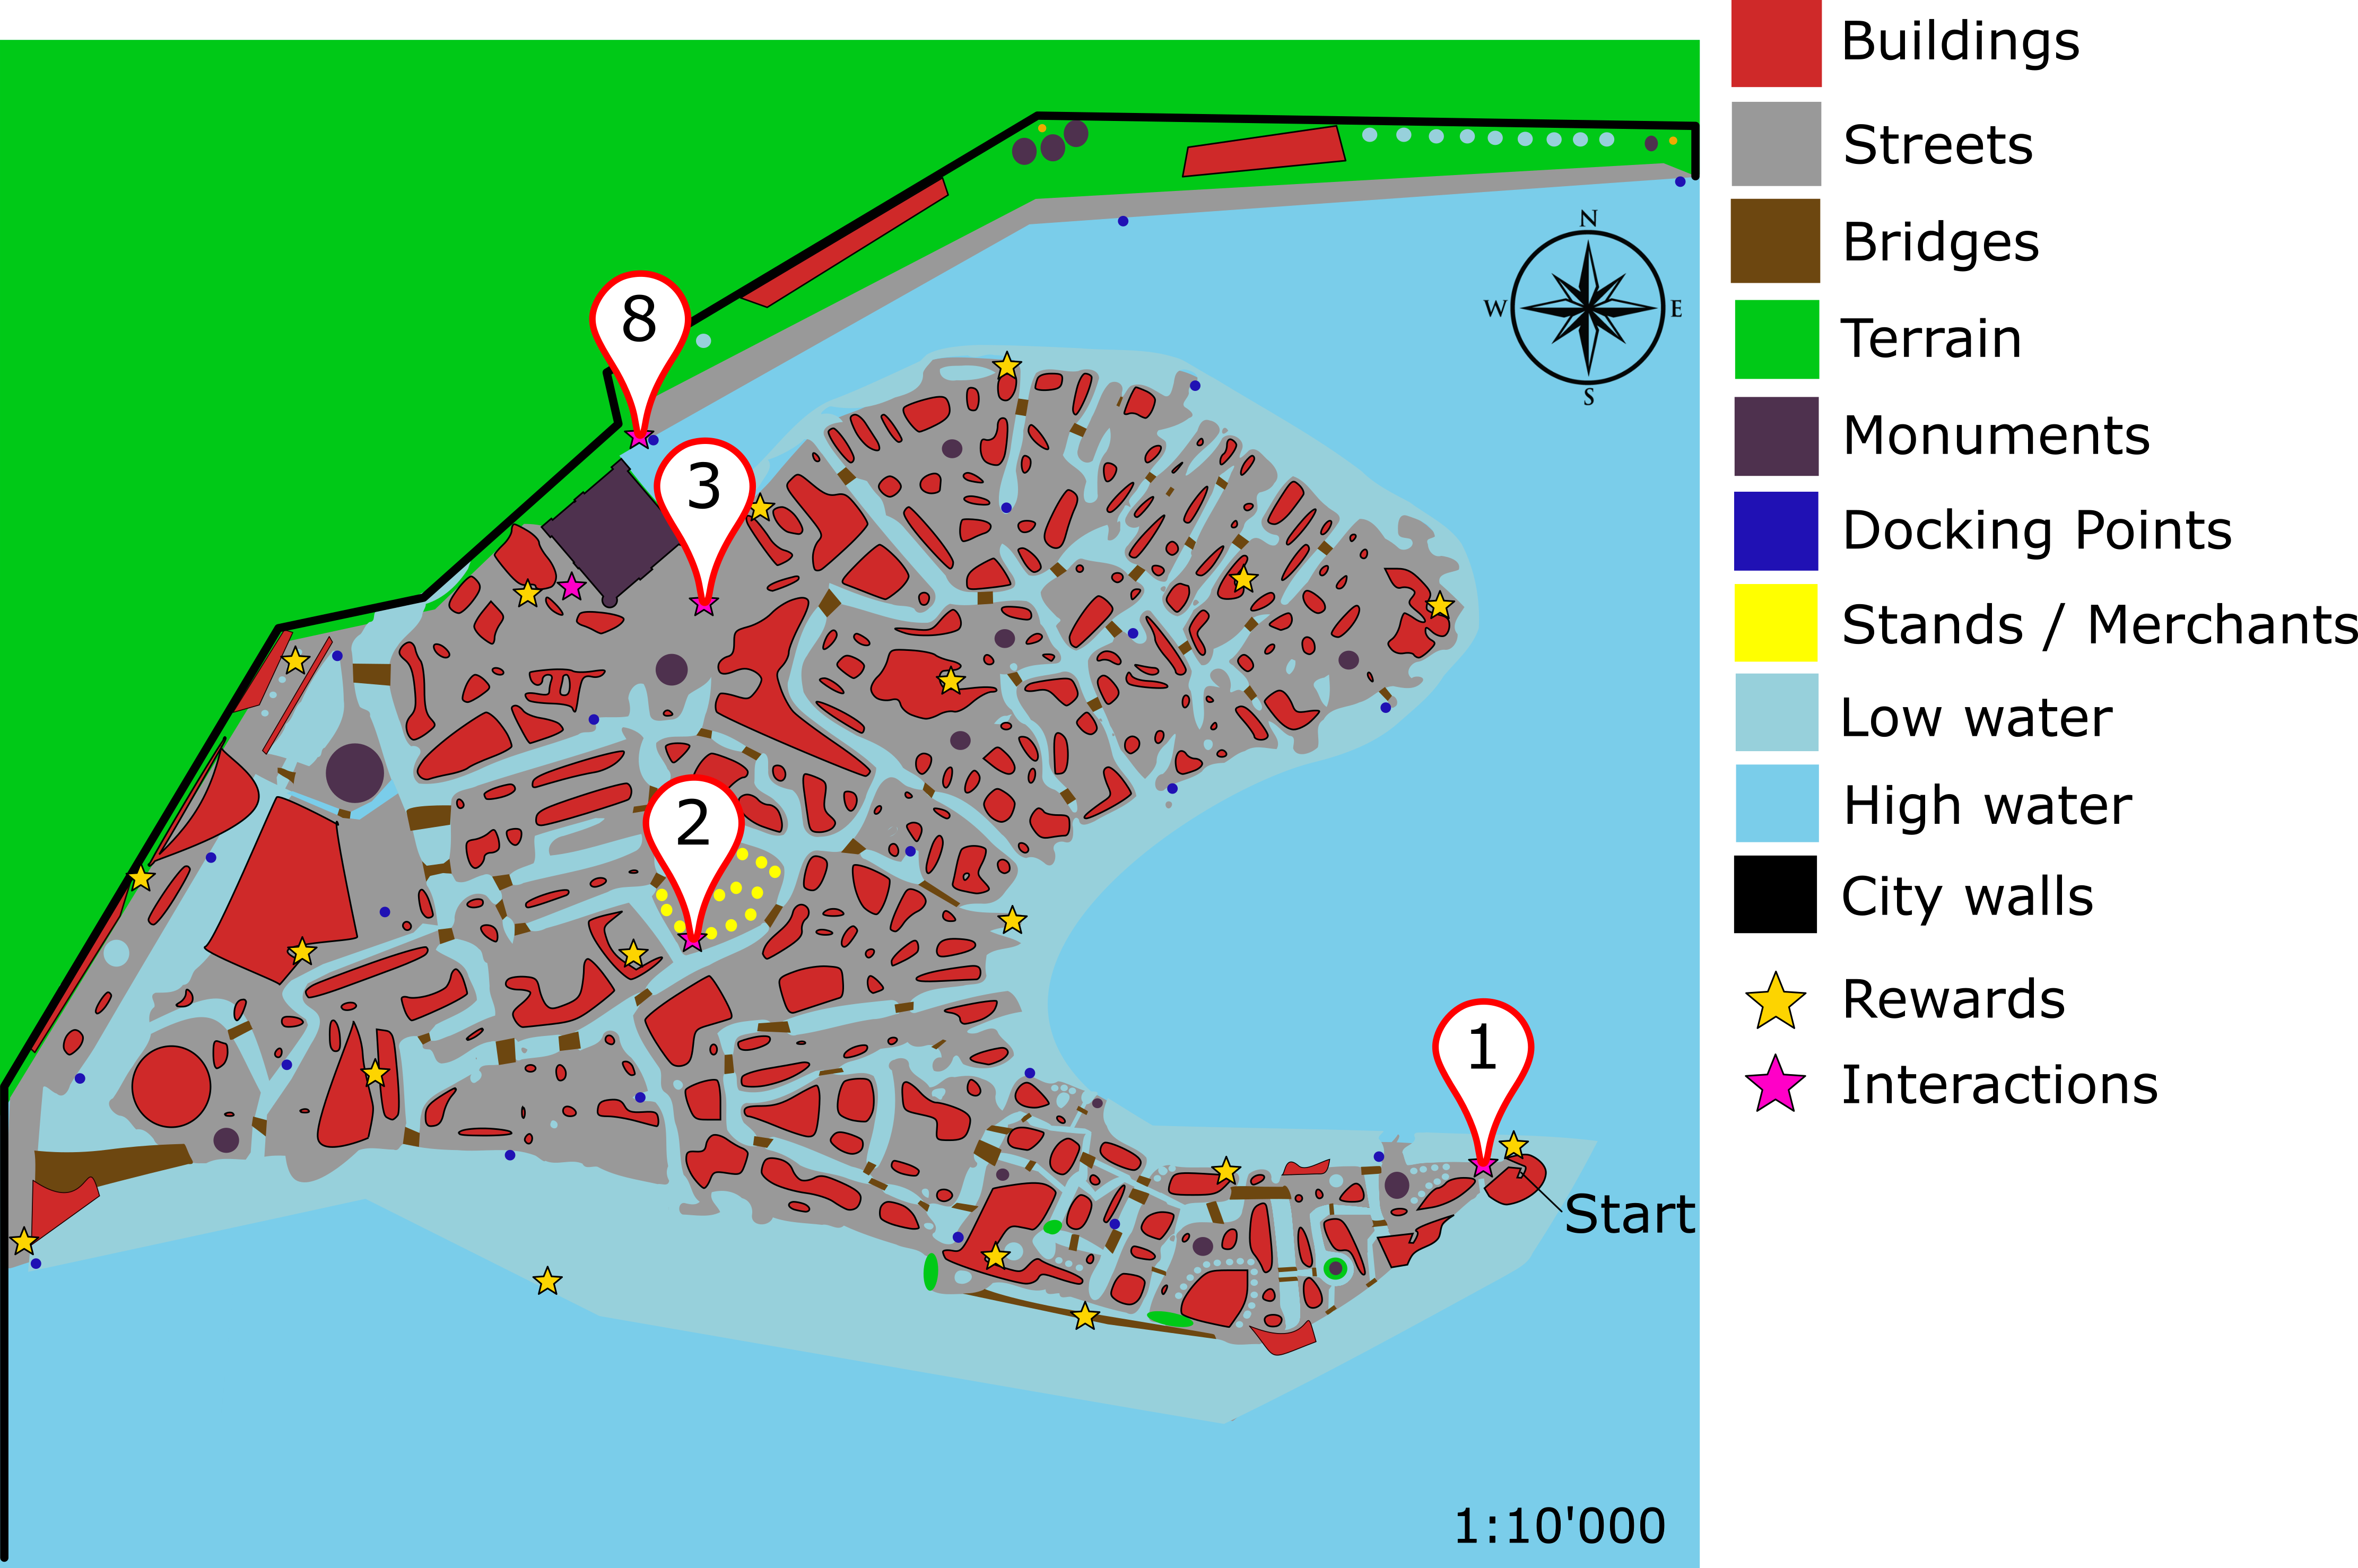
\includegraphics[scale=0.47]{Images/Maps/dynamiaCheckpoints}
  \caption{Checkpoints in the city of Dynamia}
\end{figure}
\begin{figure}[H]
  \centering
  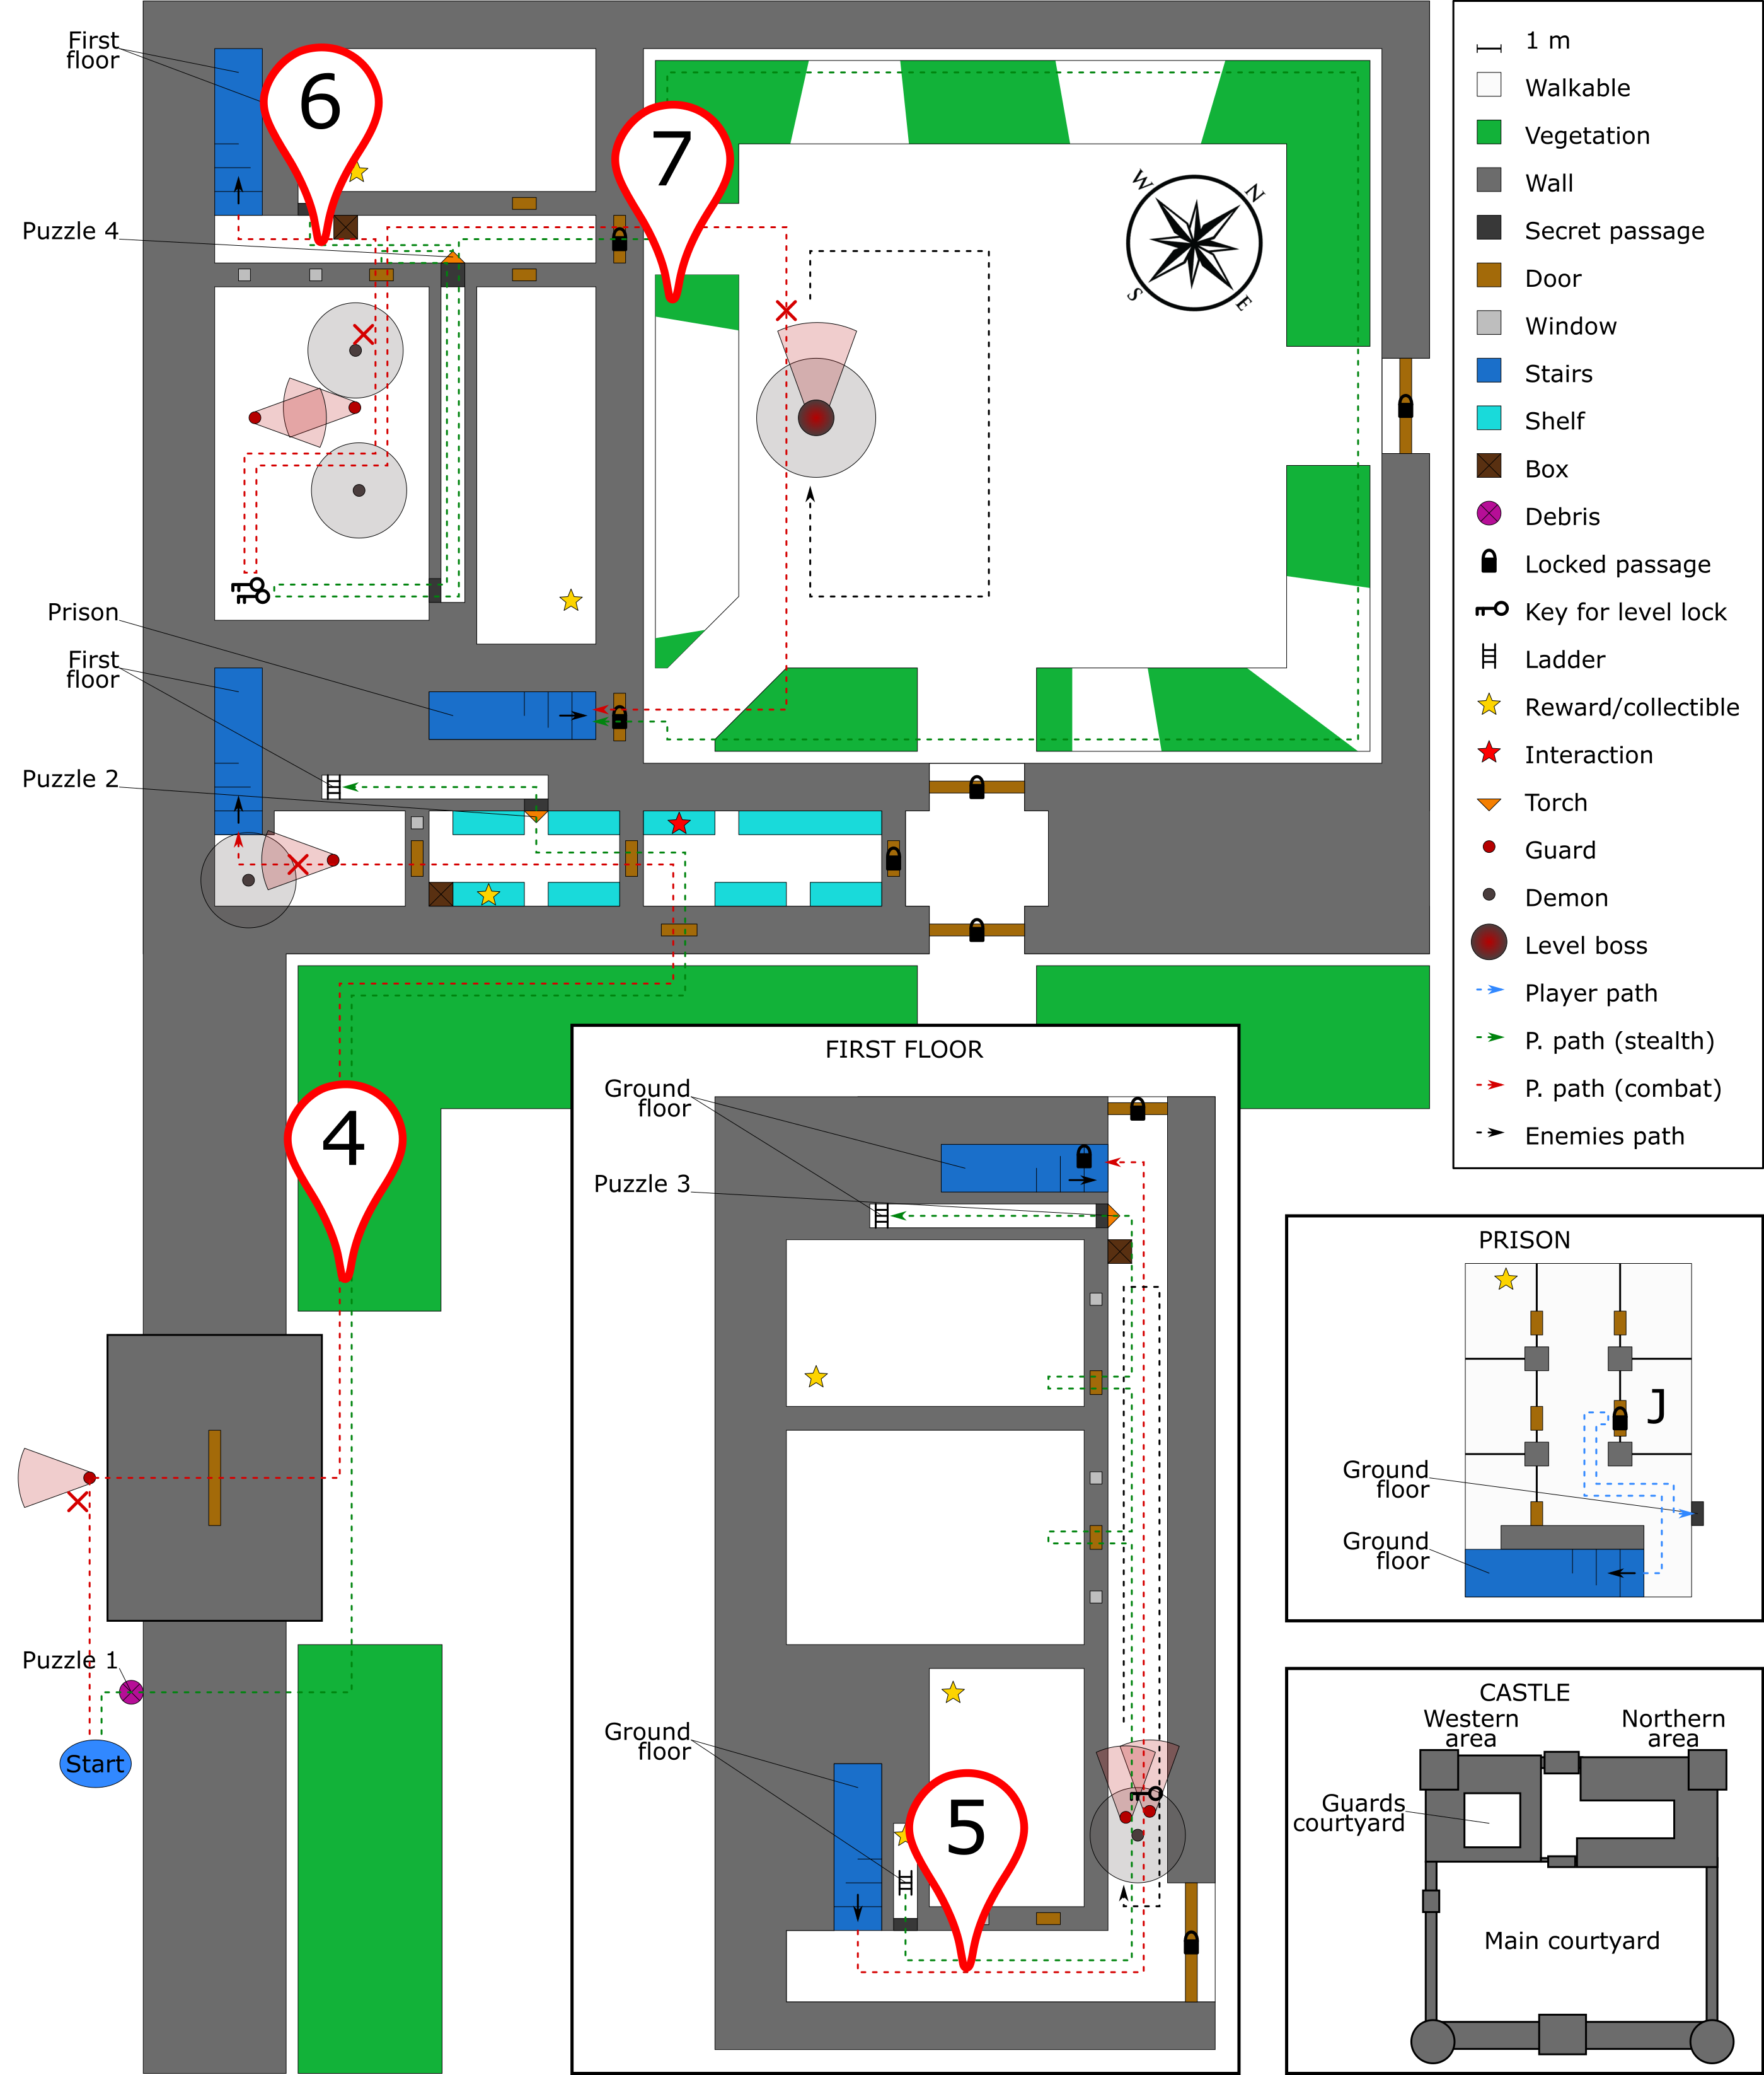
\includegraphics[scale=0.2]{Images/Maps/castleOfDynamiaCheckpoints}
  \caption{Checkpoints in the Castle of Dynamia}
\end{figure}

\begin{enumerate}
 \item The first checkpoint is immediately after Sophie talks to the map near the dead end.
 \item The second checkpoint is in the market and it will be activated once Sophie has interacted with the merchant during the main story course.
 \item The third checkpoint will be activated once Sophie has reached the square where there are the newsboys.
 \item As soon as she gets inside the castle the player will activate the fourth checkpoint.
 \item As soon as the player reaches the first floor the player will unlock his fifth checkpoint.
 \item Just before trying to defeat two guards or solving the puzzle 4  the player will get another checkpoint.
 \item The second to last checkpoint will be provided to the player in a safe zone before the encounter with the boss of the level.
 \item The last checkpoint is placed at the docking point where Sophie and her friends will take to Shark machine to get away from the guards.
\end{enumerate}
